\section{Gidrostatik bosim}

\begin{enumerate}

\item Suyuqlik bosimi formulasi: 
\begin{enumerate}[label=\Alph*)]
\item $p=mgh$
\item $p=mg$
\item $p=\rho Vg$
\item $p=\rho gh$
\end{enumerate}


\item Rasmda tasvirlangan nuqtalardagi suyuqlik bosimlarni taqqoslang.

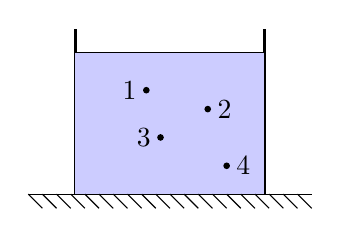
\begin{tikzpicture}[scale=0.6]

% --- idish devorlari ---
\draw[thick] (-2,0) -- (-2,3.5);
\draw[thick] (2,0) -- (2,3.5);



% --- suyuqlik ---
\fill[blue!20] (-2,0) rectangle (2,3);

% suyuqlik sathi
\draw (-2,3) -- (2,3);

% --- yer (shtrix) ---
\draw (-3,0) -- (3,0);
\foreach \x in {-3,-2.7,...,3}
{
\draw (\x,0) -- (\x+0.3,-0.3);
}

% --- nuqtalar ---
\fill ( -0.5,2.2) circle (2pt);
\node[left] at (-0.5,2.2) {1};

\fill (0.8,1.8) circle (2pt);
\node[right] at (0.8,1.8) {2};

\fill (-0.2,1.2) circle (2pt);
\node[left] at (-0.2,1.2) {3};

\fill (1.2,0.6) circle (2pt);
\node[right] at (1.2,0.6) {4};

\end{tikzpicture}

\begin{enumerate}[label=\Alph*)]
\item 4 katta, 2 kichik. 
\item 1 kichik, 4 katta. 
\item hamma bir xil. 
\item 1 katta, 2 kichik. 

\end{enumerate}


\item Idish tubiga gidrostatik bosim nimalarga bog‘liq?

1) idish shakliga; 2) idish tubining yuziga; 3) idishdagi suyuqlik zichligiga; 4) suyuqlik ustunining balandligiga.
\begin{enumerate}[label=\Alph*)]
\item 1 va 2.
\item 2 va 3.
\item 3 va 4.
\item 1 va 4.  
\end{enumerate}

\item Suyuqlikning idish tubiga bosimi ...
\begin{enumerate}[label=\Alph*)]
\item  suyuqlik zichligiga to‘g‘ri, ustunining balandligiga teskari proporsional. 
\item  suyuqlik ustuni balandligiga to‘g‘ri proporsional bo‘lib, suyuqlik zichligiga teskari proporsional. 
\item  suyuqlik ustunining balandligiga to‘g‘ri proporsional bo‘lib, suyuqlik zichligiga bog‘liq emas. 
\item  suyuqlik zichligiga va ustunining balandligiga to‘g‘ri proporsional.
\end{enumerate}

\item Qalinligi 0,5 m bo‘lgan benzin qatlami idish tubiga qanday bosim beradi(kPa)? 
Benzinning zichligi 800 kg/m$^3$.

\begin{enumerate}[label=\Alph*)]
\item 2.
\item 4.
\item 5.
\item 6.
\end{enumerate}


\item Zichligi 900 kg/m$^3$ bo‘lgan suyuqlikning 30 cm chuqurlikka ega bo‘lgan joydagi bosimini toping (Pa).

\begin{enumerate}[label=\Alph*)]
\item 2700.
\item 27000.
\item 270000.
\item 3000.
\end{enumerate}


\item Balandligi 40 m bo‘lgan suv ustunining bosimini aniqlang (kPa). Suvning zichligi 1000 kg/m$^3$, $g=10$ N/kg.

\begin{enumerate}[label=\Alph*)]
\item 4.
\item 4,5.
\item 40.
\item 400.
\end{enumerate}


\item Suvning ko‘l tubiga beradigan bosimi 200 kPa bo‘lishi uchun, ko‘lning chuqurligi qanday bo‘lishi kerak (m)?

\begin{enumerate}[label=\Alph*)]
\item 2.
\item 10.
\item 20.
\item 100.
\end{enumerate}


\item Rasmda ko‘rsatilgandek, idishlarning biriga suv, ikkinchisiga kerosin quyilgan. Idishlar tutashish joyida elastik parda bilan ajratilgan. Qaysi idish tubiga bosim kattaroq? Suyuqliklarni ajratuvchi elastik parda (ab) qaysi tomonga egiladi?

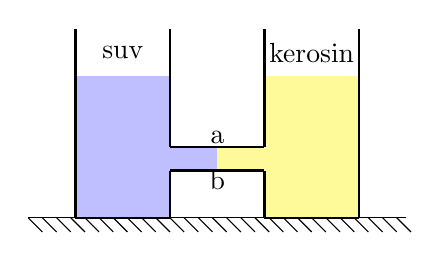
\begin{tikzpicture}[scale=0.6]

% --- chap idish (suv) ---
\fill[blue!25] (-4,0) rectangle (-2,3);
\fill[blue!25] (-2.1,1) rectangle (-1,1.5);
\node at (-3,3.5) {suv};

\draw[thick] (-4,0) -- (-4,4);
\draw[thick] (-2,0) -- (-2,1);
\draw[thick] (-2,1.5) -- (-2,4);
\draw[thick] (-4,0) -- (-2,0);


% --- o‘ng idish (kerosin) ---
\fill[yellow!40] (0,0) rectangle (2,3);
\fill[yellow!40] (-1,1) rectangle (0,1.5);
\node at (1,3.5) {kerosin};

\draw[thick] (0,0) -- (0,1);
\draw[thick] (2,0) -- (2,4);
\draw[thick] (0,1.5) -- (0,4);
\draw[thick] (0,0) -- (2,0);



% --- tutash qism (kanal) ---
\draw[thick] (-2,1.5) -- (0,1.5);
\draw[thick] (-2,1) -- (0,1);

% --- elastik parda (a, b) ---
\node at (-1,1.7) {a};
\node at (-1,0.8) {b};

% --- yer (shtrix) ---
\draw (-5,0) -- (3,0);
\foreach \x in {-5,-4.7,...,3}
{
\draw (\x,0) -- (\x+0.3,-0.3);
}

\end{tikzpicture}


\begin{enumerate}[label=\Alph*)]
\item $p_{\text{suv}}=p_{\text{ker}},$ egilmaydi.
\item $p_{\text{suv}}>p_{\text{ker}},$ suv tomonga.
\item $p_{\text{suv}}>p_{\text{ker}},$ kerosin tomonga.
\item $p_{\text{ker}}>p_{\text{suv}},$ kerosin tomonga.
\end{enumerate}



\item Turli shakldagi 3 ta idishga bir xil suyuqlik bir xil balandlikkacha quyilgan. 
Idishlar tubiga bosimlar munosabati qanday bo‘ladi?

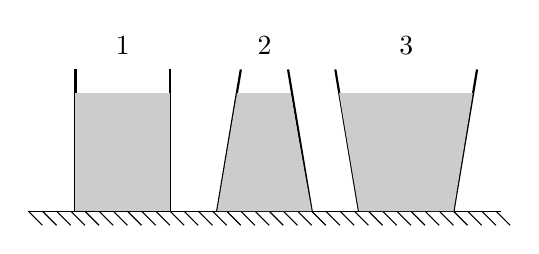
\begin{tikzpicture}[scale=0.6]

% --- yer (shtrix) ---
\draw (-1,0) -- (9,0);
\foreach \x in {-1,-0.7,...,9}
{
\draw (\x,0) -- (\x+0.3,-0.3);
}

% --- 1-idish (to‘g‘ri) ---
\draw[thick] (0,0) -- (0,3);
\draw[thick] (2,0) -- (2,3);
\draw[thick] (0,0) -- (2,0);

\fill[gray!40] (0,0) rectangle (2,2.5);
\node at (1,3.5) {1};

% --- 2-idish (toraygan) ---
\draw[thick] (3,0) -- (3.5,3);
\draw[thick] (5,0) -- (4.5,3);
\draw[thick] (3,0) -- (5,0);

\fill[gray!40] (3,0) -- (3.42,2.5) -- (4.55,2.5) -- (5,0) -- cycle;
\node at (4,3.5) {2};

% --- 3-idish (kengaygan) ---
\draw[thick] (6,0) -- (5.5,3);
\draw[thick] (8,0) -- (8.5,3);
\draw[thick] (6,0) -- (8,0);

\fill[gray!40] (6,0) -- (5.58,2.5) -- (8.41,2.5) -- (8,0) -- cycle;
\node at (7,3.5) {3};

\end{tikzpicture}

\begin{enumerate}[label=\Alph*)]
\item $p_1=p_2=p_3$.
\item $p_2>p_1>p_3$.
\item $p_1=p_3<p_2$.
\item $p_2>p_1<p_3$.
\end{enumerate}


\item Suvning idish tubiga bosim kuchi uning yon sirtiga beradigan bosim kuchiga teng bo‘lishi uchun suv to‘ldirilgan radiusi 5 cm li silindr idishning balandligi qanday bo‘lishi kerak (m)?

\begin{enumerate}[label=\Alph*)]
\item 0,5.
\item 0,1.
\item 0,05.
\item 0,8.
\end{enumerate}


\item Qanday shart bajarilganda, suyuqlikning silindrik idish tubiga bosim kuchi uning yon sirtiga bosim kuchiga teng bo‘ladi? $r$ – silindr asosining radiusi, $h$ – suyuqlikning balandligi.

\begin{enumerate}[label=\Alph*)]
\item $h=2r$.
\item $h=r$.
\item $h=\pi r$.
\item $h=\dfrac{r}{\pi}$.
\end{enumerate}


\item Asosining yuzi 1 cm$^2$ bo‘lgan silindrik idishdagi suv idish tubiga 10 kPa bosim bermoqda. Agar suvni asosi 10 marta katta bo‘lgan idishga quysak, suv avvalgi bosimni berishi uchun bu idishga yana necha litr suv quyish kerak? $\rho_{\text{suv}}=1$ g/cm$^3$, $g=10$ N/kg.

\begin{enumerate}[label=\Alph*)]
\item 9.
\item 1,8.
\item 0,45.
\item 0,9.
\end{enumerate}


\item Agar suvning idish tubiga beradigan bosimi kerosin beradigan bosimdan 
2 marta katta bo‘lsa, suv ustuni balandligining kerosin ustuni balandligiga 
nisbati nimaga teng bo‘ladi? $\rho_{\text{suv}}=1000$ kg/m$^3$, 
$\rho_{\text{ker}}=800$ kg/m$^3$.

\begin{enumerate}[label=\Alph*)]
\item 1,6.
\item 2.
\item 1.
\item 0,8.

\end{enumerate}



\end{enumerate}


\begin{table}[h!]
\centering
\begin{tabular}{|c|c|c|c|c|c|c|}
\hline
№ & J. & № & J. & № & J.  \\ \hline
1 & D & 6 & A & 11 & C \\ \hline
2 & B & 7 & D & 12 & B \\ \hline
3 & C & 8 & B & 13 & D \\ \hline
4 & D & 9 & C & 14 & A  \\ \hline
5 & B & 10 & A & 15 &   \\ \hline
\end{tabular}
\end{table}